%Formatting Report
\documentclass[12pt, a4paper]{article}

% Page margins
\usepackage[top=2.54cm, bottom=2.54cm, left=2cm, right=2cm]{geometry}

% Format Citations
\usepackage[style=phys, backend=biber]{biblatex}
\addbibresource{References.bib}

% Section title customization
\usepackage{titlesec}
\titleformat{\section}[block]{\normalfont\Large\bfseries}{\thesection}{1em}{}  % Larger section titles

% Adjust paragraph indentation and spacing
\setlength{\parindent}{0pt}  % No Indentation for paragraphs
\setlength{\parskip}{0pt}     % No extra space between paragraphs
\usepackage[skip=3pt]{parskip}



%word count commands:
\newcommand{\detailtexcount}[1]{%
  \immediate\write18{texcount -merge -sum -q #1.tex output.bbl > #1.wcdetail }%
  \verbatiminput{#1.wcdetail}%
}

\newcommand{\quickwordcount}[1]{%
  \immediate\write18{texcount -1 -sum -merge -q #1.tex output.bbl > #1-words.sum }%
  \input{#1-words.sum} words%
}

\newcommand{\quickcharcount}[1]{%
  \immediate\write18{texcount -1 -sum -merge -char -q #1.tex output.bbl > #1-chars.sum }%
  \input{#1-chars.sum} characters (not including spaces)%
}



% Change caption font size
\usepackage{caption}
\DeclareCaptionFont{tenpt}{\fontsize{10}{12}\selectfont}
\captionsetup[figure]{font=tenpt}

%General 
\usepackage{graphicx}
\usepackage{braket}
\usepackage{subcaption}
\usepackage{titlesec}
\usepackage{xcolor}
\usepackage{hyperref}
\usepackage{array}
\usepackage{amsmath}
  
\begin{document}
%Title Page
\begin{center}
\vspace*{\stretch{1}}

{\Large \textbf{Development of an Ultra-Efficient Single-Photon \\ Sources at Room Temperature for Quantum Communication Applications} \\[\stretch{2}]}


\textsc{CID: 02209727 \\ Word Count: XXX}\\[\stretch{2}]

\begin{figure}[hb!t]
     \centering
     \begin{subfigure}[b]{0.5\textwidth}
         \centering
         
\includegraphics[width=\textwidth]{Title/ICL_Logo.jpg}
     \end{subfigure}
     ~\\[1 cm]
     \begin{subfigure}[b]{0.5\textwidth}
         \centering
         
\includegraphics[width=\textwidth]{Title/UAM_Logo.jpg}
     \end{subfigure}
     \hfill
\end{figure}

~\\[1cm]

\textsc{A thesis submitted \\[1ex]
to \\[1ex]
Faculty Of Science, Imperial College London\\[\stretch{3}]}

\textsc{Supervisor}\\[2ex]

\begin{tabular}[t]{@{}c@{}}
\bfseries Prof. Dr. Carlos Antón-Solanas \\
Departamento de Física de Materiales\\
Facultad de Ciencia \\
Universidad Autónoma de Madrid
\end{tabular}\hfil

\vspace*{\stretch{3}}

\end{center}

\newpage





%Preface
\begin{center}
    \Large{\textbf{Preface}} \\
\end{center}
~\\[0.5 cm]

Speak about the general COMPHORT group, their goals and what aspect UAM (and hence I) is focusing on.
Preface identifying precisely what your part in the work has been, and what was done by others. 

\newpage

%Contents
\begingroup
\titleformat{\section}[block]{\Large\bfseries\filcenter}{\color{red}}{}{}
\tableofcontents
\vspace{24 pt}
\endgroup
\newpage

%Abstract
\begin{center}
    \Large{\textbf{Abstract}} \\
\end{center}
~\\[0.5 cm]

\textbf{Abstract (in two languages) which clearly and concisely identifies the principal features of the work and the results achieved}

\newpage

%Introduciton
\section{Introduction}

This work investigates the non-resonant excitation of hexagonal boron nitride (hBN) defects at room temperature to achieve bright and pure single-photon emission. Additionally, Purcell enhancement is pursued by coupling the single-photon modes to an open plano-concave Fabry-Pérot cavity.

Efficient single-photon production is critical for advancing quantum technologies, with applications ranging from enhancing measurement precision beyond classical limits \cite{Nagata2007, Vitelli2010} to enabling reliable transport and processing of analogue information in photonic circuits \cite{Bogaerts2020}. Among these applications, quantum key distribution (QKD) is the most mature, leveraging the quantum properties of single photons to detect eavesdropping attempts and create secure communication channels. 

The first QKD protocol proposed was BB84 \cite{Bennett2014}, in which Alice (the sender) transmits photons polarised in one of two bases: the rectilinear basis ($\ket{H}$, and $\ket{V}$) or the diagonal basis ($\ket{D}=(\ket{H}+\ket{V})/\sqrt{2}$, and $\ket{A}=(\ket{H}-\ket{V})/\sqrt{2}$). These states encode binary bits (0 or 1) in two mutually unbiased bases. For each photon, Bob (the receiver) randomly selects a basis for measurement (either rectilinear or diagonal) and, after detection, publicly announces which basis was used, without revealing the measured bit value. Alice and Bob then retain only the results where they chose the same basis, using them to construct a shared secret key.

If an eavesdropper (Eve) intercepts and measures a photon, she must randomly select a basis, with a $ \frac{1}{2} $ probability of choosing incorrectly. When she measures in the wrong basis, the quantum state collapses into an incorrect polarization. If she resends the photon, it remains in the wrong state with probability $ \frac{1}{2} $, introducing an error in Bob’s measurement. Alice and Bob detect Eve by comparing $ n $ bits of their shared key. The probability of Eve measuring each photon in the correct basis by chance is $\left(\frac{1}{2}\right)^n$, which decreases exponentially with $n$, allowing security to be arbitrarily strengthened.

While BB84 is provably secure against eavesdropping in an idealised quantum setting \cite{Shor2000}, a significant weakness arises when multi-photon pulses are used instead of true single-photon sources. In such cases, Eve can exploit the photon-number splitting (PNS) attack \cite{Ashkenazy2024} by using a beam splitter to measure one of the transmitted photons while allowing the other to continue to Bob undisturbed. This allows her to extract information about the key without introducing detectable errors, highlighting the necessity of true single-photon sources for ensuring secure quantum communication.

\subsection{Benchmarking Single-Photon Sources}

An ideal single-photon source should emit exactly one photon on demand, with each photon possessing identical characteristics. To assess the quality of a single-photon source, three key parameters are evaluated: Purity ($P$), Indistinguishability ($I$), and Brightness ($B$). For an ideal source, all three parameters reach their maximum value, such that $ P = I = B = 1 $.

\subsubsection{\label{sec:purity} Purity}
Purity is a loss-independent measure that quantifies the likelihood that the source emits only one photon at a time. It is defined as $P = 1 - g^{(2)}(0)$, where $g^{(2)}(0)$ is the second-order correlation function at zero time delay. The function $g^{(2)}(\tau)$ describes the statistical correlation between detecting two photons separated by a time delay $\tau$ relative to a completely random (Poissonian) photon distribution:

\begin{equation}
    g^{(2)}(\tau) = \frac{\langle I(t)I(t+\tau)\rangle}{\langle I(t)\rangle^2},
    \label{eqn:g2}
\end{equation}

where $\langle \rangle$ denotes a time-averaged quantity, and $I(t)$ is the measured photon intensity at time $t$. For an ideal single-photon emitter, $g^{(2)}(0) = 0$, indicating perfect antibunching, meaning that photons are emitted strictly one at a time, with no possibility of multi-photon events. In contrast, coherent light (such as from a laser) follows Poissonian statistics and has a $g^{(2)}(0) = 1$ (\textcolor{red}{Potentially show this mathematically}), which indicates no correlation between photon detections. A value of $g^{(2)}(0) > 1$ is characteristic of bunched light, such as thermal sources, where photons tend to arrive in clusters due to bosonic bunching effects. In practice, achieving $g^{(2)}(0) < 0.5$ is a strong indicator of a non-classical light source, supporting potential single-photon emission. This measurement is typically performed using a Hanbury Brown and Twiss (HBT) interferometer \cite{Brown1956}.

\subsubsection{Indistinguishability}

Indistinguishability, also a loss-independent measure, quantifies the likelihood that two photons will interfere in a Hong-Ou-Mandel (HOM) setup \cite{Hong1987}. The Hong-Ou-Mandel effect states that when two indistinguishable photons arrive simultaneously at the input ports of a 50:50 beam splitter, they will always exit together through the same output port, rather than taking separate paths \cite{Hong1987}.

\textcolor{red}{----------Potentially Remove----------}

The degree of indistinguishability of a single-photon source is typically assessed by measuring the $g^{(2)}(0)$, often denoted $g^{(2)}_{\text{HOM}}(0)$, at the output of a path-unbalanced Mach-Zehnder interferometer \cite{Rarity2024}. One arm of the interferometer includes a delay line matched to the temporal separation between sequential photons. To achieve a perfect temporal overlap of consecutive photons, a pulsed laser, typically with a pulse width on the order of 3 ps, much shorter than the temporal envelope of the single photons (which is typically several nanoseconds at room temperature), is used for alignment. The laser is passed into the interferometer and one of the output ports of the second beam splitter is sent to a spectrometer. When the laser pulses are not temporally overlapped, a spectral beating pattern is observed due to partial interference. In contrast, perfect temporal alignment results in a Gaussian-shaped spectral feature.

The indistinguishability can be approximately expressed as $ I \approx 1 - 2g^{(2)}_{\text{HOM}}(0) $. This relation is only approximate because it assumes the source emits exactly one photon per pulse. In practice, multi-photon emission and other imperfections can affect the measured indistinguishability. The expression becomes exact in the ideal case of a perfect single-photon source with no multi-photon contributions. The factor of two arises from the fact that, for a pure but fully distinguishable photon source, $ g^{(2)}_{\text{HOM}}(0) = 0.5 $, as the two photons have a 50\% probability of exiting the same output port of the beam splitter. 

\textcolor{red}{--------------------------------------}

For two photons to be indistinguishable, they must occupy the same spatial mode, have identical spectral and temporal profiles, and be in equivalent polarisation and phase states \cite{Senellart2017}. The spatial mode refers to the spatial distribution of the photon wavepacket; typically, single-mode optical fibres are used to ensure that photons are collected into the same well-defined optical mode. Spectral indistinguishability is determined by the line-width of the emitter, while the temporal profile is governed by the emitter’s lifetime, $T_1=1/\gamma$. Polarisation indistinguishability requires that the photons have the same polarisation orientation, which can be ensured using polarisers and wave plates. The phase coherence of single photons describes the stability of their phase over time, which determines their ability to interfere consistently in quantum optics experiments. The length of time over which the phase is stable is quantified by the pure dephasing time, given by $T_2^*=1/\gamma^*$ and which can be measured using a Michelson interferometer \cite{Michelson1887, Jelezko2003}. 


\subsubsection{Brightness}

The brightness describes the probability that a single photon is emitted per excitation pulse. Unlike $P$ and $I$, brightness is a loss-dependent measure, as it depends on the detection efficiency and optical setup. Therefore, when comparing sources, it is important to distinguish between the brightness at the source ($B_s$), measured before any optical losses, and the detected brightness ($B_d$), which is affected by transmission losses, collection efficiency and detector efficiency. For meaningful comparisons, experimental setups must carefully characterise and account for losses throughout the optical system.

The brightness of single-photon sources can be enhanced by making use of cavity quantum electrodynamic effects. When an emitter is placed inside an optical cavity, an additional decay channel is introduced alongside the bare radiative decay rate, $\gamma_r$, and the non-radiative decay rate, $\gamma_{nr}$. The emitter can now emit into the optical cavity mode via a Jaynes–Cummings-type interaction characterised by a coherent coupling rate $g$. The cavity then emits this energy into the external environment at a rate given by the cavity linewidth, $\kappa$. In the weak coupling regime, defined by $2g \ll \kappa$, the combined decay rate of the emitter becomes $\gamma' = \gamma_r + \gamma_{nr} + R$, where $R = \frac{4g^2}{\kappa + \Gamma}$ is the effective rate of emission through the cavity mode, and $\Gamma$ is the full width at half maxima of the emitter.

If the cavity spectral width is much greater than that of the emitter ($\kappa \gg \Gamma$), the decay rate simplifies to $\gamma' = \gamma + \gamma_r F_P$, where $F_P$ is the Purcell factor given by $F_P = \frac{4g^2}{\kappa \gamma_r}$. Importantly, the cavity coupling rate $g$ and decay rate $\kappa$ are functions of the cavity mode volume $V$ and quality factor $Q$, respectively. As a result, the Purcell factor $F_P \propto Q/V$ depends solely on the cavity design and is independent of the emitter itself. The $Q$-factor of a cavity quantifies how well the cavity stores energy, and is defined as the ratio of the cavities resonant frequency to the linewidth of the emitter.

Examples of emitters exhibiting Purcell enhancement include semiconductor quantum dots embedded in a micro pillar cavities \cite{Engel2023}, and organic dye molecules placed in the near field of a specially designed plasmonic nanoantenna \cite{Zhao2020}. 

\subsection{Types of Single-photon Source}

\subsubsection{Probabilistic Single-photon Sources}

Probabilistic single-photon sources based on nonlinear optical processes, such as spontaneous parametric down-conversion (SPDC) and four-wave mixing (FWM) \cite{Chopin2023}, have historically been the most widely used methods for generating single photons. These sources are termed probabilistic because, for each pump pulse, there is a probability of producing zero, one, or multiple photon pairs. When exactly one pair is generated, detection of one photon, referred to as the idler, heralds the presence of its partner, the signal, which can then be used as a single-photon source.

The quantum state of light emitted from such a source can be modelled as a two-mode squeezed vacuum state \cite{Braunstein2005}:

\begin{equation}
\begin{aligned}
    |\psi\rangle &= \sqrt{1 - |\lambda|^2} \sum_{n=0}^{\infty} \lambda^n  \ket{n}\ket{n} \\
    &= \sum_{n=0}^{\infty} p_n \ket{n}\ket{n},
    \label{eqn:squeezed_state_model}
\end{aligned}
\end{equation}

where $|\lambda|^2 = \tanh^2(r)$ and $r$ is a dimensionless squeezing parameter proportional to the pump laser power. In an ideal scenario where it is possible to resolve the number of photons in the idler arm \cite{Davis2022, Sempere-Llagostera2022a}, all multi-photon events can be discarded, resulting in a signal state with unit purity. However, under this idealised condition, the brightness of the source has a fundamental upper bound of $B = 1/4$.

In practice, most setups do not employ photon-number-resolving detectors in the idler arm and can only register whether any photons are detected. When such a detection occurs, the vacuum component of the signal mode is eliminated, and the heralded state collapses to a statistical mixture of multi-photon Fock states with $n \geq 1$. The resulting density matrix of the signal mode is given by:

\begin{equation}
    \rho = \sum_{n=1}^{\infty} \frac{|p_n|^2}{\sum_{k=1}^{\infty} |p_k|^2} \ket{n}\bra{n},
    \label{eqn:density_matrix_SPDC}
\end{equation}

where the denominator ensures proper normalisation over the non-vacuum components.

The purity of the heralded signal state can be found using a rewritten version of the second-order correlation function:

\begin{equation}
\begin{aligned}
    g^{(2)}(0) &= \frac{\langle \hat{n}(\hat{n} - 1) \rangle}{\langle \hat{n} \rangle^2} \\
    &= \frac{\langle \hat{a}^\dagger \hat{a}^\dagger \hat{a} \hat{a} \rangle}{\langle \hat{a}^\dagger \hat{a} \rangle^2} \\
    &= \frac{\mathrm{Tr}(\rho \hat{a}^\dagger \hat{a}^\dagger \hat{a} \hat{a})}{\left[\mathrm{Tr}(\rho \hat{a}^\dagger \hat{a})\right]^2},
\end{aligned}
\end{equation}

where the number operator $\hat{n}$ has been expressed in terms of the photon creation ($\hat{a}^\dagger$) and annihilation ($\hat{a}$) operators. By inserting equation~\ref{eqn:density_matrix_SPDC} and evaluating the relevant matrix elements using the Fock state relations $\hat{a} \ket{n} = \sqrt{n} \ket{n-1}$ and $\hat{a}^\dagger \ket{n} = \sqrt{n+1} \ket{n+1}$, one finds that the second-order correlation function to be $g^{(2)}(0) = 2|\lambda|^2$. Therefore, the purity, as defined in section~\ref{sec:purity}, scales with pump strength as:

\begin{equation}
    P = 1 - 2\tanh^2(r).
\end{equation}

In contrast, the brightness of the source follows the relation:

\begin{equation}
    B = \frac{\tanh^2(r)}{\cosh^2(r)},
\end{equation}

which increases with pump power. This illustrates a fundamental trade-off between brightness and purity in probabilistic sources \cite{Senellart2017}, imposing limitations on the realisation of bright, high-purity single-photon emission. Recent work has focused on mitigating this limitation by synchronising multiple probabilistic sources within a fast optical switching network to realise an effective deterministic single-photon source \cite{Meyer-Scott2020}. However, this approach requires significant resources and introduces substantial cost and experimental complexity.


\subsubsection{Deterministic Single-photon Sources}

Deterministic single-photon sources leverage the discrete electronic structure of solid-state emitters, analogous to those found in natural atoms. Typically, a laser pulse is used to excite the emitter from its ground state to a higher-energy excited state. A single photon is then emitted during the spontaneous relaxation back to the ground state, enabling controlled and on-demand photon generation.

However, in solid-state systems, these emitters are embedded within a surrounding lattice, which introduces non-radiative decay channels such as vibrations. These mechanisms compete with radiative relaxation, introducing photon dephasing which reducing both the emission efficiency and the coherence of the emitted photons. The total decay rate of solid-state sources can be expressed as the sum of radiative and non-radiative contributions: $1/T_1 = \gamma_{\mathrm{rad}} + \gamma_{\mathrm{nrad}}$. The impact of non-radiative processes is characterised by the quantum efficiency, $\eta_{\mathrm{QE}}$, defined as:

\begin{equation}
    \eta_{\mathrm{QE}} = \frac{\gamma_{\mathrm{rad}}}{\gamma_{\mathrm{rad}} + \gamma_{\mathrm{nrad}}},
\end{equation}

where $\gamma_{\mathrm{rad}}$ and $\gamma_{\mathrm{nrad}}$ are the radiative and non-radiative decay rates, respectively. To experimentally determine the quantum efficiency, a method originally introduced by Drexhage is often employed \cite{Tews1970, Drexhage1968}. This approach exploits the fact that varying the distance between the emitter and a mirror modifies the local optical density of states, thereby changing $\gamma_{\mathrm{rad}}$ while leaving $\gamma_{\mathrm{nrad}}$ unaffected. By measuring changes in the total decay rate as a function of emitter–mirror separation, the quantum efficiency can be extracted.

Recent advancements in solid-state single-photon sources have focused on improving emission purity, brightness, and coherence length. Quantum dots are nanoscale semiconductor particles—commonly made from materials such as cadmium selenide (CdSe), indium phosphide (InP), or lead halide perovskites—with tunable optical emission. Under suitable excitation conditions, they can function as single-photon emitters by confining excitons and releasing individual photons. They are considered the state-of-the-art quantum emitters, with values of $g^{(2)}(0)$ reported as low as $9.4\times 10^{-5}\pm 1.9\times 10^{-3}$ \cite{Hanschke2018}. However, QDs require cryogenic temperatures and are affected by inhomogeneous broadening due to fabrication-related disorder.

Monolayer transition metal dichalcogenides (TMDCs), such as WSe$_2$, have emerged as promising alternatives due to their strong exciton binding energies and atomically thin nature. Strain-induced localisation of excitons has enabled site-controlled single-photon emission. Branny et al.\ achieved arrays of quantum emitters with a positioning accuracy of $120 \pm 32$~nm and near-unity yield~\cite{Branny2017}. These emitters exhibited high single-photon purity, with $g^{(2)}(0)$ values as low as $0.05\pm0.04$, as reported by Parto et al.~\cite{Parto2021}. TMDC-based emitters offer electrical tunability and high spatial confinement, but their performance remains limited by cryogenic operating conditions and spectral diffusion caused by interactions with the substrate and local environment.

Hexagonal boron nitride (hBN), first identified by Tran et al.~\cite{Tran2016}, is a wide-bandgap van der Waals material that hosts optically stable defect-based single-photon emitters capable of operating at room temperature. These emitters have demonstrated strong antibunching behaviour, with reported second-order correlation values as low as $g^{(2)}(0) = 6.4\times10^{-3}$ \cite{Vogl2021}, under pulsed excitation at cryogenic temperatures. Although they show variability in spectral characteristics, recent improvements in defect engineering and material growth have led to enhanced emission consistency, supporting their potential for scalable quantum photonics.



\subsection{\label{sec:source_prep}hBN Preparation: Fabrication and Excitation}

\subsubsection{Fabrication Methods}

Hexagonal boron nitride (hBN) consists of boron and nitrogen atoms arranged in a hexagonal lattice. Within each atomic layer, atoms are bonded by strong covalent interactions, while adjacent layers are held together by weaker van der Waals forces. This structure results in an atomically flat, chemically stable, and electrically insulating material with a wide bandgap of approximately 6~eV. Due to these properties, hBN is widely used as a substrate for two-dimensional materials in electronic and optoelectronic devices.

In its monolayer form, hBN exhibits a direct bandgap, making it suitable for hosting a range of point defects that can act as stable sources of single photons. Although multilayer hBN has an indirect bandgap, most research on hBN-based single-photon emitters focuses on defects within multilayer structures. These defect states are strongly spatially confined (on the order of 2--3\,\AA), and their formation and emission properties are not inhibited by the indirect nature of the bandgap.

Several techniques have been developed to fabricate single-photon emitters in hBN, each with its own trade-offs in emitter quality, spatial control, and scalability. 

\textcolor{red}{Discuss with Carlos what fabrication methods to discuss: anneahling, electron irradiation...}





\subsubsection{Excitation Schemes}

When considering excitation schemes for solid-state single-photon emitters, there are two main categories: resonant and non-resonant excitation. Each approach offers distinct advantages and disadvantages, and the best choice depends on the specific requirements of the application. To understand the principles and implications of these schemes, it is necessary to consider the expected spectral characteristics of solid-state emitters.

The emission spectrum of a solid-state emitter can generally be decomposed into two main components: the zero-phonon line (ZPL) and the phonon sideband (PSB). The ZPL appears as a higher-energy, more spectrally prominent feature and corresponds to photons emitted during a purely radiative transition from the excited state directly to the ground state, without any phonon involvement. In contrast, the PSB is a broader, lower-energy component that arises when the excited electron relaxes non-radiatively to a vibrational sublevel near the ground state. This process involves coupling to lattice phonons, resulting in photon emission that is redshifted relative to the ZPL and broadened due to phonon interactions.

Resonant excitation schemes require that the energy of the excitation laser is tuned to match the energy of the zero-phonon line (ZPL). In this case, the emitter is driven directly into its excited state and the excitation probability can be controlled by adjusting the laser power. However, because the excitation and emission wavelengths are identical, isolating the emitted photon from the excitation laser poses a significant experimental challenge.

To suppress the laser background in the collection path, polarisation and spatial filtering techniques are commonly used. One approach involves exciting the emitter with a polarised laser pulse and placing a polariser in the collection path oriented orthogonally to the excitation polarisation. Alternatively, the excitation and collection paths can be arranged in different spatial directions to reduce scattered laser light. Both methods involve trade-offs between excitation efficiency and collection efficiency, as stricter filtering reduces the amount of collected signal photons. In many resonantly driven experiments, this filtering is so stringent that the ZPL itself is blocked, and only photons from the phonon sideband are collected, which can limit indistinguishability and overall source performance.

Non-resonant excitation schemes involve pumping the emitter using a laser with energy much higher than that of the zero-phonon line (ZPL). Following excitation, the electron rapidly relaxes non-radiatively to the excited state through phonon-mediated processes, after which it decays radiatively to the ground state, emitting a single photon. This approach offers a simple and robust excitation mechanism, as it does not require precise spectral alignment with the ZPL and enables straightforward filtering using a single long-pass filter placed between the excitation laser and the ZPL.

However, the use of high-energy excitation introduces several drawbacks. The additional relaxation steps can lead to timing jitter in the photon emission and broaden the temporal profile of the wavepacket, which in turn degrades photon indistinguishability. Despite these limitations, non-resonant schemes remain widely used due to their experimental simplicity and higher collection efficiency. In this work, non-resonant excitation was employed due to limited access to a tunable-wavelength laser.

Another important consideration in the excitation scheme is whether to use pulsed or continuous-wave (CW) excitation. Pulsed excitation is preferred in most quantum technologies, as it enables precise control over the temporal spacing of photon emission, critical in quantum communication and computation protocols. In this work, both excitation schemes are considered, depending on the specific requirements of each measurement.



\subsection{Comparative Analysis of Solid-State Emitter Properties}

\subsubsection{\label{sec:coherence-time} Coherence Time}

The timescale over which an emitter produces indistinguishable photons is known as the coherence time, $T_2$, and is given by:

\begin{equation}
    \frac{1}{T_2} = \frac{1}{T_2^*} + \frac{1}{2T_1},
    \label{eqn:coherence_time}
\end{equation}

where $T_1$ is the emitter lifetime and $T_2^*$ is the pure dephasing time. In the absence of any pure dephasing mechanisms (i.e., when $1/T_2^* = \gamma^* = 0$), the emitter is said to be Fourier transform-limited, and the spectral linewidth is Lorentzian, determined solely by the spontaneous emission rate, with a full width at half maximum ($\Gamma$) given by $ = 1/T_1 = \gamma$. In this ideal case, \textcolor{red}{no phase averaging occurs between subsequent photon emissions, and the emitter should produce perfectly indistinguishable photons}; an essential requirement for quantum interference-based applications such as linear optical quantum computing and boson sampling.

In practice, however, this idealised case is rarely realised due to the presence of spectral wandering and phonon-induced dephasing. Even at low temperatures, where phonon interactions are suppressed, the ZPL exhibits inhomogeneous broadening due to slow spectral diffusion. This results from local fluctuations in the electric field, which cause shifts in the emission centre wavelength, leading to a more Gaussian-like lineshape. This contribution has been shown to depend on the excitation power, with a significant increase in inhomogenous broadening seen at saturation power \cite{White2021}. At high (room) temperatures the $\Gamma$ broadening depends on $T^3$ \cite{Sontheimer2017, White2021, Horder2022}, where $T$ is temperature, showing a strong dephasing due to phonon coupling. Such fast phonon dephasing mechanics contribute a homogenous broadening to the spectrum, and the lineshape develops a Lorentzian contribution with $\Gamma = 2/T_2$. 

The indistinguishability of a source can crudely be approximated by $I\approx T_2/(2T_1)$. Values for this ratio vary significantly across solid-state emitter platforms and is strongly dependent on the host material, operating temperature and excitation scheme.

\textcolor{red}{Ask Carlos about the measuremtns for T2, some use fits other use Michelson???}

hBN cryo (4 K): $I\approx 0.4$ \cite{Fournier2023}???\\
hBN cryo (4 K): $I\approx 0.008$ \cite{Sontheimer2017}\\
hBN cryo: $I\approx 0.2$ \cite{Horder2022} \\
TMDC cryo (4 K): $I\approx 0.003$ \cite{vonHelversen2023}\\
QD"s: $I\approx 0.956$ \cite{Ulhaq2010} no Michelson??\\

\textcolor{red}{Include maths showing the exponential decay of phase}

\subsubsection{Quantum Efficiency and Debye-Waller Factor}

Although the coherence time of an emitter is the most important factor when considering its suitability for use in quantum technologies, other numerical quantities such as the quantum efficiency and Debye-Waller factor should be taken into account. The Debye-Waller factor, $DW$, quantifies the fraction of photons emitted without phonon coupling, and is defines as:

\begin{equation}
    DW=\frac{I_{ZPL}}{I_{TOTAL}},
\end{equation}

where $I_{ZPL}$ and $I_{TOTAL}$ is the intensity of the ZPL and whole emission spectrum, respectively. 

hBN DW: $0.82$ \cite{Tran2016} at cryo \\
TMDC DW: $0.4$ \cite{Micevic2022} \\
QD DW: up to $0.743$ \cite{Chen2025} \\


\subsection*{Extra paragraphs}

1) Despite extensive efforts to engineer reliable deterministic single-photon sources \cite{Eisaman2011}, no simple and stable source has yet been developed with the necessary properties for practical implementation.As a result, attenuated lasers are commonly used to generate weak coherent states \cite{Stucki2005}. However, these sources follow a Poissonian photon number distribution, meaning there is always a nonzero probability of emitting multi-photon pulses, leaving them vulnerable to PNS attacks. While security-enhancing protocols, such as decoy state QKD \cite{Lo2005}, have been introduced to mitigate this risk, recent studies have demonstrated that even imperfect sub-Poissonian photon sources can outperform state-of-the-art weak coherent state lasers in secure quantum communication \cite{Ordan2024}.



\newpage


%Experimental Method
\section{Experimental Methods}

\begin{itemize}
    \item Setup: Micro-photoluminescence in confocal configuration 
    \begin{itemize}
        \item Lasers (CW or pulsed), and their characterisation. Discuss elliptical Gaussian beam and optimisation program
        \item Detectors (spectrometer + CCD or APD's)
        \item Non-resonant excitation (Carlos' review)
    \end{itemize}
    \item Imaging techniques
    \begin{itemize}
        \item Wide non-resonant excitation of sample + CCD
        \item APD scans with fiber
        \item Coordinate system to locate defects
    \end{itemize}
    \item Cavity coupling 
    \begin{itemize}
        \item Cavity system + techniques 
        \item Q-factor, mesas, micro-mirrors \& lenses
        \item k-space imaging 
        \item White light reflectivity
    \end{itemize}
    \item Lifetime measuremeants and how they are done
    \item $g^{(2)}(0)$ and HBT measurements
\end{itemize}

%Results
\section{Results and Discussion}

\subsection{hBN in the Absence of a Cavity}

Choose 2/3 defects and include all the following

\subsubsection{Emitter Characteristics}

1) Include big 2x2 graphic with lifetime, spectrum, g2(0), Saturation Curve.

\subsubsection{Power and Filter Dependent Dephasing Rate}

2) Visibility against time-delay (dephasing rate)




\subsection{Cavity Measurements}

\subsubsection{k-Space and Newton Ring Characterisation}

\subsubsection{Reflectivity Measurements}



\subsection{Integration of hBN Emitters with an Open Fabry–Pérot Cavity}

Explain the limitations of why we were not able to do this


%Conclusion
\section{Conclusion}
i) discuss to what extent the aims of the project, given earlier, have been achieved

ii) state what further work would be appropriate

%Appendix
\section{Appendix \label{sec:appendix}}

\subsubsection*{Bottom Mirror Transmittance}

The transmittance spectrum of the base mirror, consisting of 10 DBR layer pairs, is shown in Fig.~\ref{fig:trans}. The stopband spans from approximately 1.6~eV to 2.2~eV or 560~nm to 775~nm.

\begin{figure}[h]
    \centering
    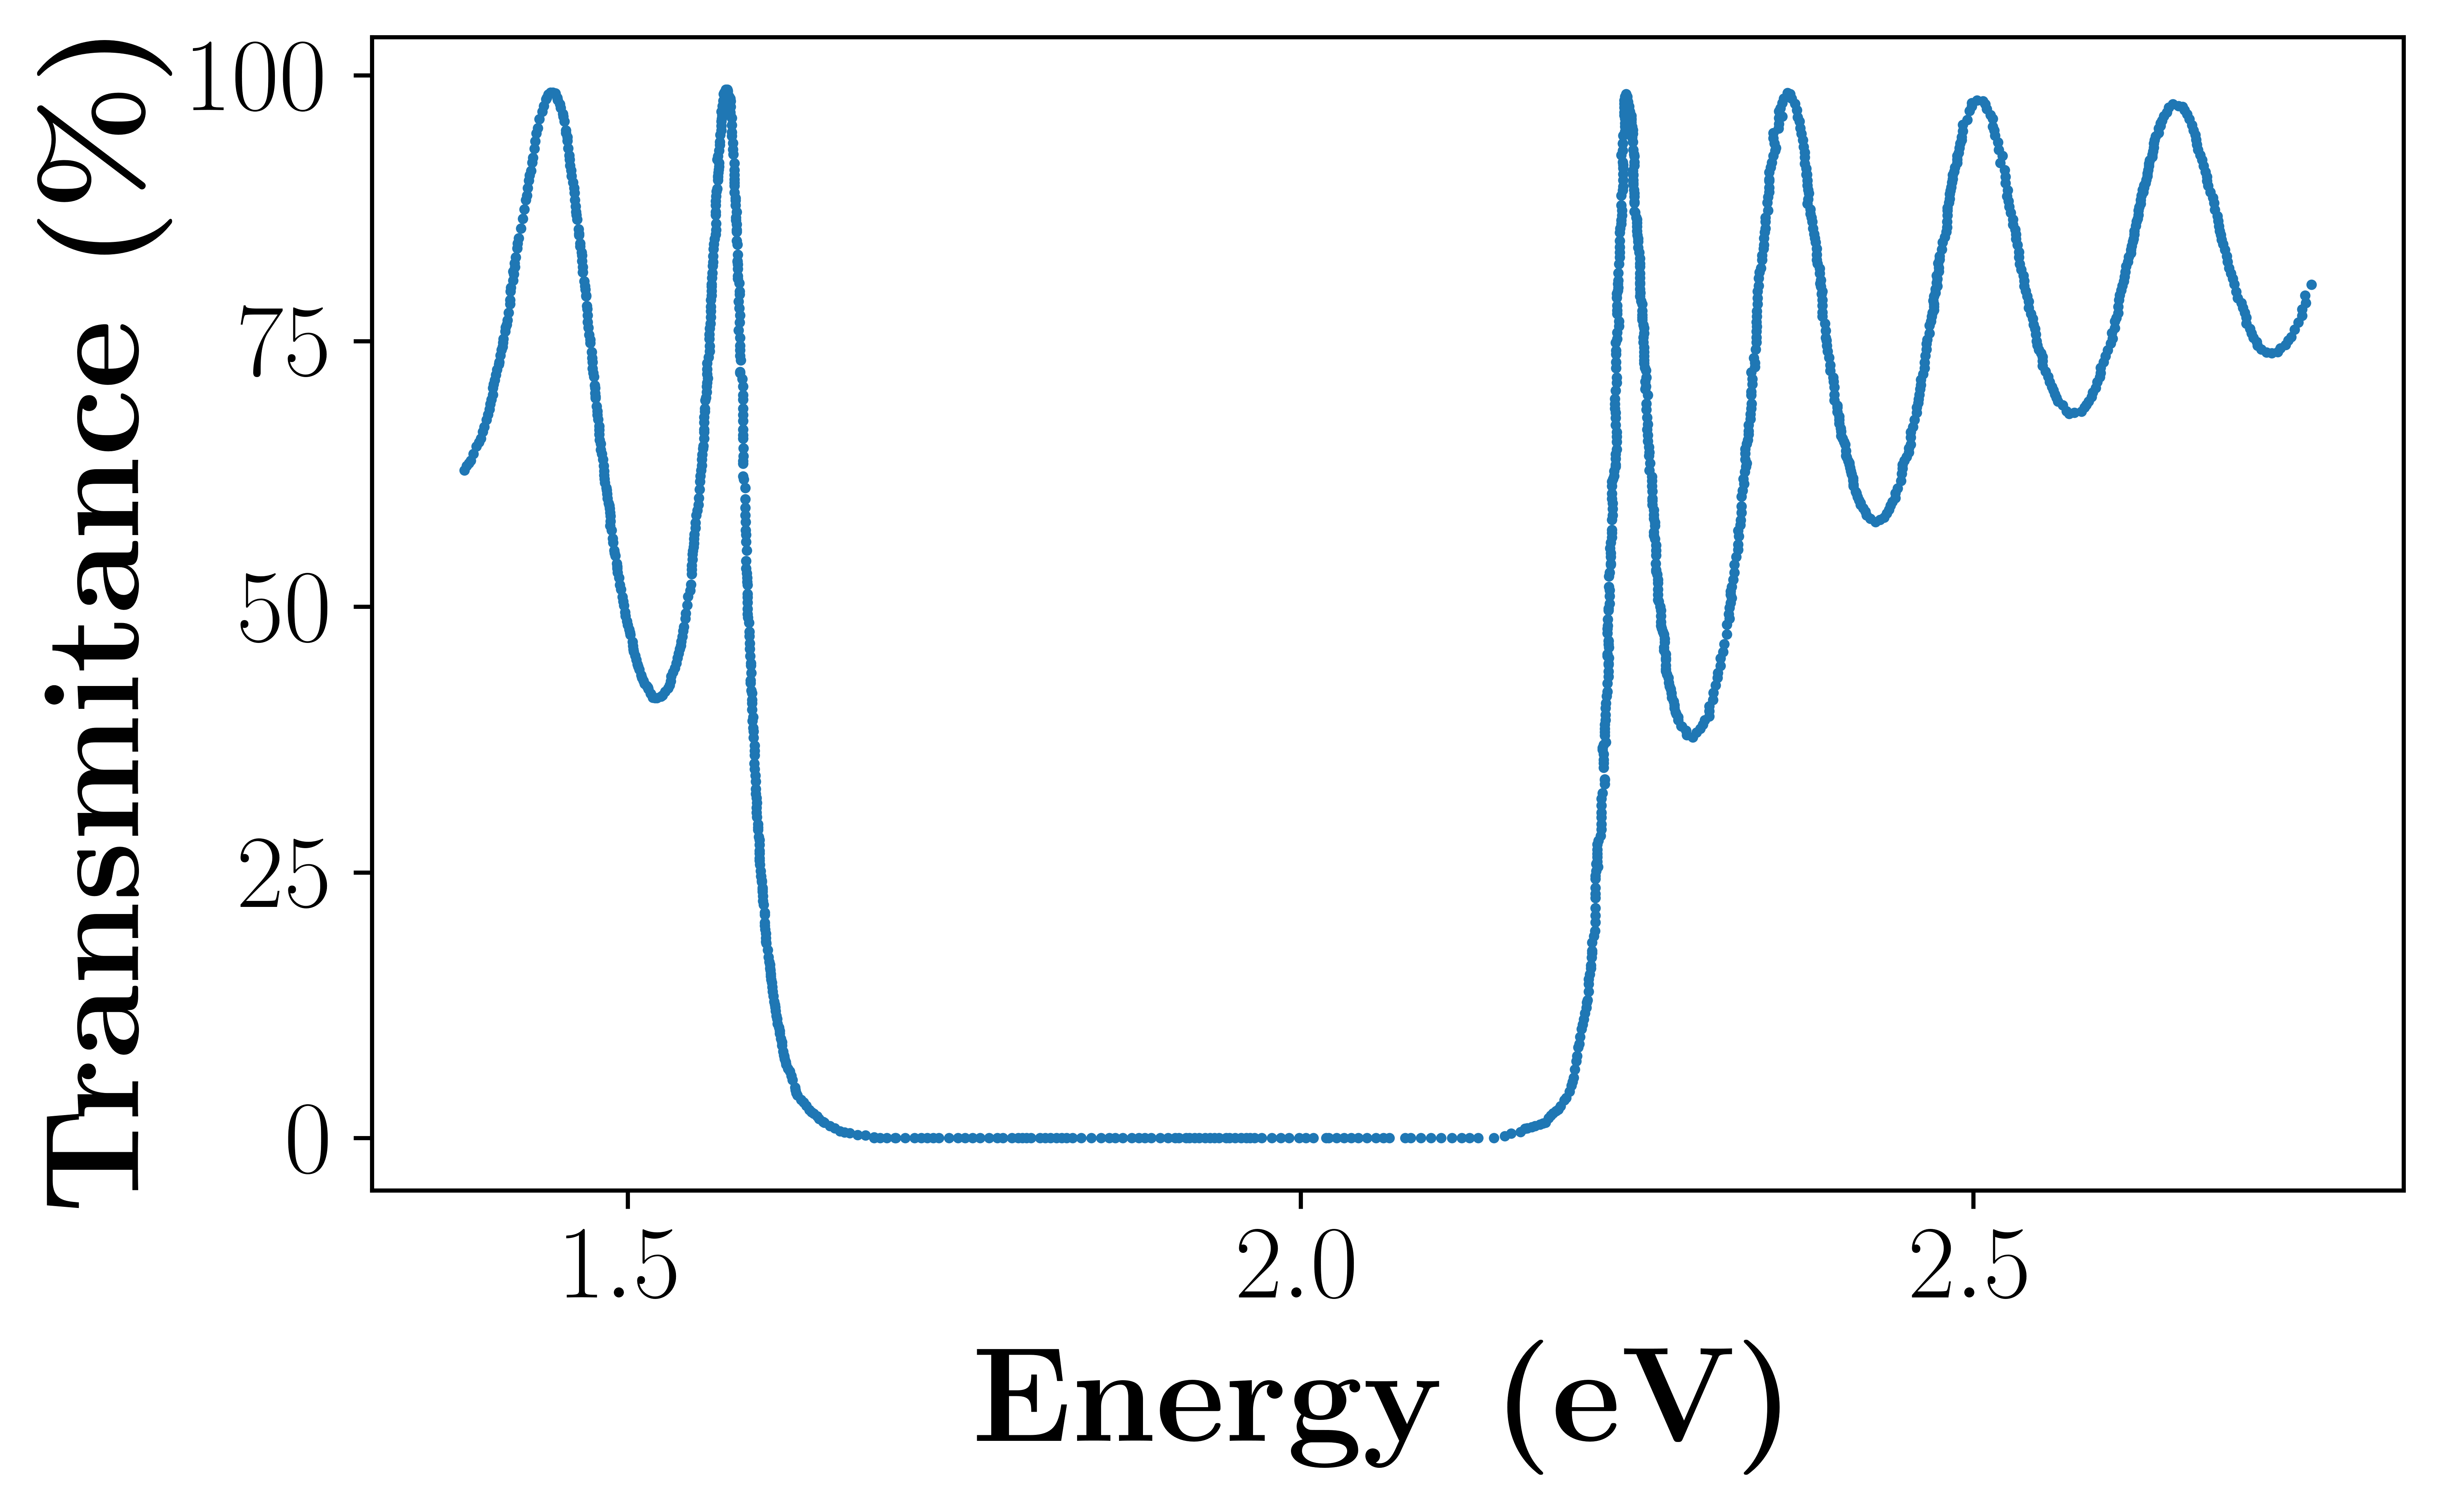
\includegraphics[width=0.5\linewidth]{Figures/Transmitance.png}
    \caption{Transmittance spectrum of the bottom DBR mirror with 10 layer pairs. The shaded region corresponds to the photonic stopband between 1.6~eV and 2.2~eV.}
    \label{fig:trans}
\end{figure}

\printbibliography
\addcontentsline{toc}{section}{References}
\end{document}
